\section{Homework 1} 

\begin{prob}
   Write down the definition of \textbf{independence} of two \textbf{events}.  
\end{prob}
\begin{solution}
    Two events $A,B$ are \textbf{independent} if $P(A\cap B)=P(A)P(B)$.
\end{solution}
\begin{prob}
    Write down the definition of the \textbf{cumulative distribution function} of a random variable.
\end{prob}
\begin{solution}
        For any random variable $X$, the \textbf{cumulative distribution function} of $X$ is a function $F_X \colon \R \to [0,1] $, where $F_X (x) = \P[X \leq x]$ for all $x \in \R$.
\end{solution}

\begin{prob}
    Let $\Omega= \{a_1,a_2,a_3,a_4,a_5\} $ be an outcome space, and let $\P$ be a probability on $\Omega$. Assume that $\P[A] = 0.5, \P [B] = 0.4, \P[C]=0.4$, and $\P [D]=0.2$, where \[
    A = \{a_1,a_2,a_3\},\ B=\{a_2,a_3,a_4\},\ C =\{a_3,a_5\} ,\ D=\{a_4\} .
    \] Are the events $A$ and $B$ independent? Why?
\end{prob}
\begin{solution}
    They are not independent, since their intersection in the outcome space is non-empty.
\end{solution}

\begin{prob}
Show that the probability of rolling two sixes twice is just as likely as rolling two threes twice.    
\end{prob}
\begin{solution}
    Rolling die are independent events as well as each double dice roll, so the probability of rolling two sixes twice is equivalent to the probability of rolling a dice 4 times in a row and getting 6 each time. By the multiplication rule for independent events we have \[
        P(6 \cdot 6 \cdot  6 \cdot  6)=P(6)P(6)P(6)P(6)=\frac{1}{6^4}=\frac{1}{1296}.
    \] Similarly, \[
        P(3 \cdot 3 \cdot  3 \cdot  3)=P(3)P(3)P(3)P(3)=\frac{1}{3^4}=\frac{1}{1296}.
    \] So the probabilities of the two events are equal.
\end{solution}

\begin{prob}
If you roll a pair of fair dice, what are the probabilities of    
\begin{enumerate}[label=(\arabic*)]
\setlength\itemsep{-.2em}
    \item Getting a sum of 1?
    \item Getting a sum of 5?
    \item Getting a sum of 12?
\end{enumerate}
\end{prob}
\begin{solution}
        Think of the sample space as the space of ordered pairs $S= \{(m,n) \mid m,n \in \{1,\cdots ,6\} \} $ representing the ordered die tosses. Then $|S|=36$.
    \begin{enumerate}[label=(\arabic*)]
    \setlength\itemsep{-.2em}
        \item There are no two integers in $\{1,\cdots ,6\} $ that sum up to 1. So this probability is zero.
        \item The pairs of integers summing up to 5 in $\{1,\cdots ,6\} $ are $(1,4)$ and $(2,3)$. Since order of tossing matters we have the four possibilities $(1,4),(4,1),(2,3),(3,2)$, and the probability of getting a sum of 5 is $\frac{4}{36}=\frac{1}{9}$.
        \item The only pair of integers summing up to 12 in $\{1,\cdots ,6\} $ are $(6,6)$. So the probability of getting a sum of 6 is $\frac{1}{36}$.
    \end{enumerate}
\end{solution}


\begin{prob}
    Problem 3.8 from the textbook.
\end{prob}
\begin{solution}
    \begin{enumerate}[label=(\alph*)]
    \setlength\itemsep{-.2em}
\item Living below the poverty line and speaking a foreign language are not disjoint. Let $A$ represent living below the poverty line and  $B$ represent speaking a foreign language. Then $P(A \cap B)=0.042\neq 0$, so these two outcomes are not disjoint.
\item The variables $A$ and $B$ are the same as in the previous part.
\begin{figure}[H]
\centering
 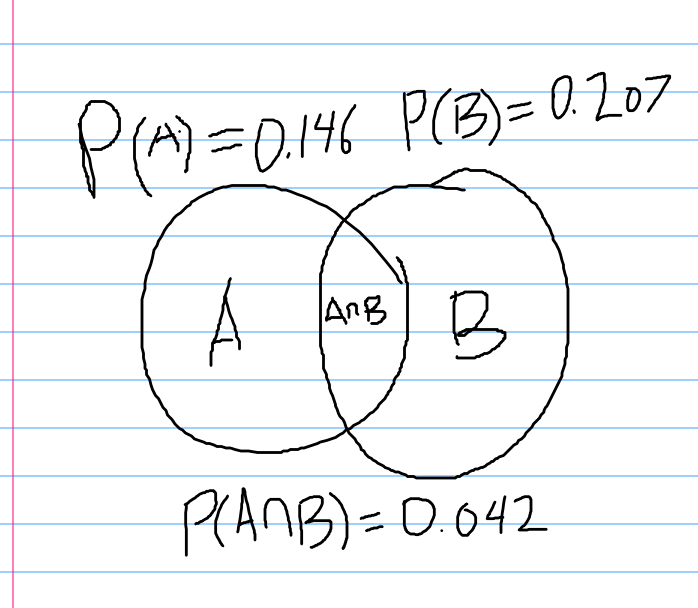
\includegraphics[width=0.4\linewidth]{hw_figures/hw1_poverty.png}
\caption{The events and their associated probabilities.}
\label{hw1_poverty}
\end{figure}
\item The percentage of Americans living below the poverty line only speaking English is $14.6-4.2=10.4$ percent.
\item The percentage of Americans living below the poverty line or speak a foreign language is $14.6+20.7-4.2=31.1$ percent.
\item The percentage of Americans living above the poverty line only speaking English is $1-31.1=68.9$ percent.
\item The event that someone lives below the poverty line is not independent of the event that the person speaks a foreign language at home. If they were, we would have \[
        P(A \cap B)=P(A)P(B)=0.030222.
    \] However, we know that $P(A \cap B)=0.042$. So the assumption that the two conditions are independent must be false.
    \end{enumerate}
\end{solution}

\begin{prob}
    Problem 3.20 as in the textbook.
\end{prob}
\begin{solution}
    We know that $P(\text{condition} \mid +)=P(\text{condition} \cap +)/P(+)$. Drawing out the tree, we have $P(\text{condition} \cap +)=0.03*0.99=0.0297.$ Then we have $P(+)=0.0297+0.97*0.02=0.0491$. Dividing, we get $P(\text{condition} \mid +)=0.0297/0.0491=0.604888$.
\end{solution}

\begin{prob}
   Problem 3.22 as in the textbook. 
\end{prob}
\begin{solution}
    The answer is 0.4867. See Figure 2 for the steps.
    \begin{figure}[H]
    \centering
     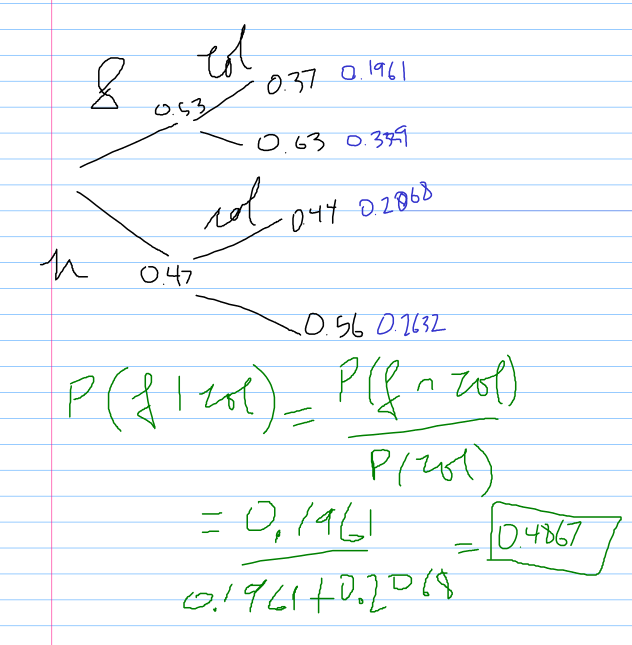
\includegraphics[width=0.6\linewidth]{hw_figures/hw1_voting.png}
    \label{hw1_voting}
    \caption{Problem 3.22 work.} 
    \end{figure}
\end{solution}
